\documentclass{article}
\usepackage[utf8]{inputenc}
\usepackage{amsmath}
\usepackage{graphicx}
\graphicspath{ {./images/} }
\usepackage{hyperref}

\title{RL Excercise Chapter 2}
\author{huseyinabanox }
\date{June 2022}

\begin{document}

    \maketitle
    \setcounter{section}{1}


    \section{Exercises}

    \subsection{Question}
    In \(\epsilon\)-greedy action selection, for the case of two actions and \(\epsilon = 0.5 \), what is the probability that the greedy action is selected?

    \subsection*{Answer}

    0.5

    \subsection{Question}

    Bandit example Consider a k-armed bandit problem with k = 4 actions, denoted 1,
    2, 3, and 4. Consider applying to this problem a bandit algorithm using \(\epsilon\)-greedy action selection,
    sample-average action-value estimates, and initial estimates of Q1(a) = 0, for all a. Suppose the initial
    sequence of actions and rewards is A1 = 1, R1 = 1, A2 = 2, R2 = 1, A3 = 2, R3 = 2, A4 = 2, R4 = 2,
    A5 = 3, R5 = 0. On some of these time steps the \(\epsilon\) case may have occurred, causing an action to be
    selected at random. On which time steps did this definitely occur? On which time steps could this
    possibly have occurred?

    \subsection*{Answer}

    \begin{table}[]
        \begin{tabular}{llllllll}
            t & Q(A1) & Q(A2) & Q(A3) & Greedy & Selected & Reward & Random?  \\
            0 & 0     & 0     & 0     & Any    & 1        & 1      & Yes      \\
            1 & 1     & 0     & 0     & 1      & 2        & 1      & Yes      \\
            2 & 1     & 1     & 0     & 1,2    & 2        & 2      & Yes      \\
            3 & 1     & 3/2   & 0     & 2      & 2        & 2      & Probable \\
            4 & 1     & 5/3   & 0     & 2      & 2        & 2      & Probable \\
            5 & 1     & 7/3   & 0     & 2      & 3        & 0      & Yes
        \end{tabular}
    \end{table}

    Random action selection may result in the selection of greedy action. Thus all steps may involved random action selection.

    If greedy action and selected actions are different then random selection is certain.

    \subsection{Question}

    In the comparison shown in Figure 2.2, which method will perform best in the long run in
    terms of cumulative reward and probability of selecting the best action? How much better will it be?
    Express your answer quantitatively.

    \subsubsection*{Answer}

    Average reward for \(\epsilon\) = 0.1 seems to be flatten while average reward for \(\epsilon\) = 0.01 is still improving. In the long run method with \(\epsilon\) = 0.01 will probably perform better.

    In terms of selecting best action; \(\epsilon\) = 0.01 selects greedy action 10 times more frequently than \(\epsilon\) = 0.1.

    \subsection{Question}
    f the step-size parameters, \(\alpha_n\), are not constant, then the estimate \(Q_n\) is a weighted
    average of previously received rewards with a weighting different from that given by (2.6). What is
    the weighting on each prior reward for the general case, analogous to (2.6), in terms of the sequence of
    step-size parameters?

    \subsubsection*{Answer}

    \begin{equation}
        Q_{n+1}=Q_{n}+\alpha_{n}[R_n-Q_n]=\alpha_{n}R_n+(1-\alpha_{n})Q_n
    \end{equation}

    \begin{equation}
        Q_{n+1}=\alpha_{n}R_n+(1-\alpha_{n})[Q_{n-1}+\alpha_{n-1}[R_{n-1}-Q_{n-1}]]=\alpha_{n}R_n+(1-\alpha_{n})[\alpha_{n-1}R_{n-1}+(1-\alpha_{n-1})Q_{n-1}]
    \end{equation}

    \begin{equation}
        Q_{n+1}=\alpha_{n}R_n+(1-\alpha_{n})\alpha_{n-1}R_{n-1}+ (1-\alpha_{n}) (1-\alpha_{n-1})Q_{n-1}
    \end{equation}

    \begin{equation}
        Q_{n+1}=\alpha_{n}R_n+(1-\alpha_{n})\alpha_{n-1}R_{n-1}+ (1-\alpha_{n}) (1-\alpha_{n-1})[\alpha_{n-2}R_{n-2}+(1-\alpha_{n-2})Q_{n-2}]
    \end{equation}

    \begin{equation}
        Q_{n+1}=\alpha_{n}R_n+(1-\alpha_{n})\alpha_{n-1}R_{n-1}+ (1-\alpha_{n}) (1-\alpha_{n-1})\alpha_{n-2}R_{n-2}+(1-\alpha_{n}) (1-\alpha_{n-1})(1-\alpha_{n-2})Q_{n-2}
    \end{equation}

    \begin{equation}
        Q_{n+1}=\sum_{i=0}^{n-1} \alpha_{n-i}R_{n-i} \prod_{k=0}^{i-1}(1-\alpha_{n-k}) + Q_1 \prod_{i=0}^{n-1}(1-\alpha_{n-i})
    \end{equation}

    \subsection{Question}

    In the comparison shown in Figure 2.2, which method will perform best in the long run in
    terms of cumulative reward and probability of selecting the best action? How much better will it be?
    Express your answer quantitatively.

    \subsubsection*{Answer}
    A modified version of the 10-armed testbed from \href{https://github.com/LyWangPX/Reinforcement-Learning-2nd-Edition-by-Sutton-Exercise-Solutions}{https://github.com/LyWangPX} is used.

    First two bandits do not make random walk. Last two bandits make random walk.

    Constant step size performs better in case of random walk which creates a non-stationary target.

    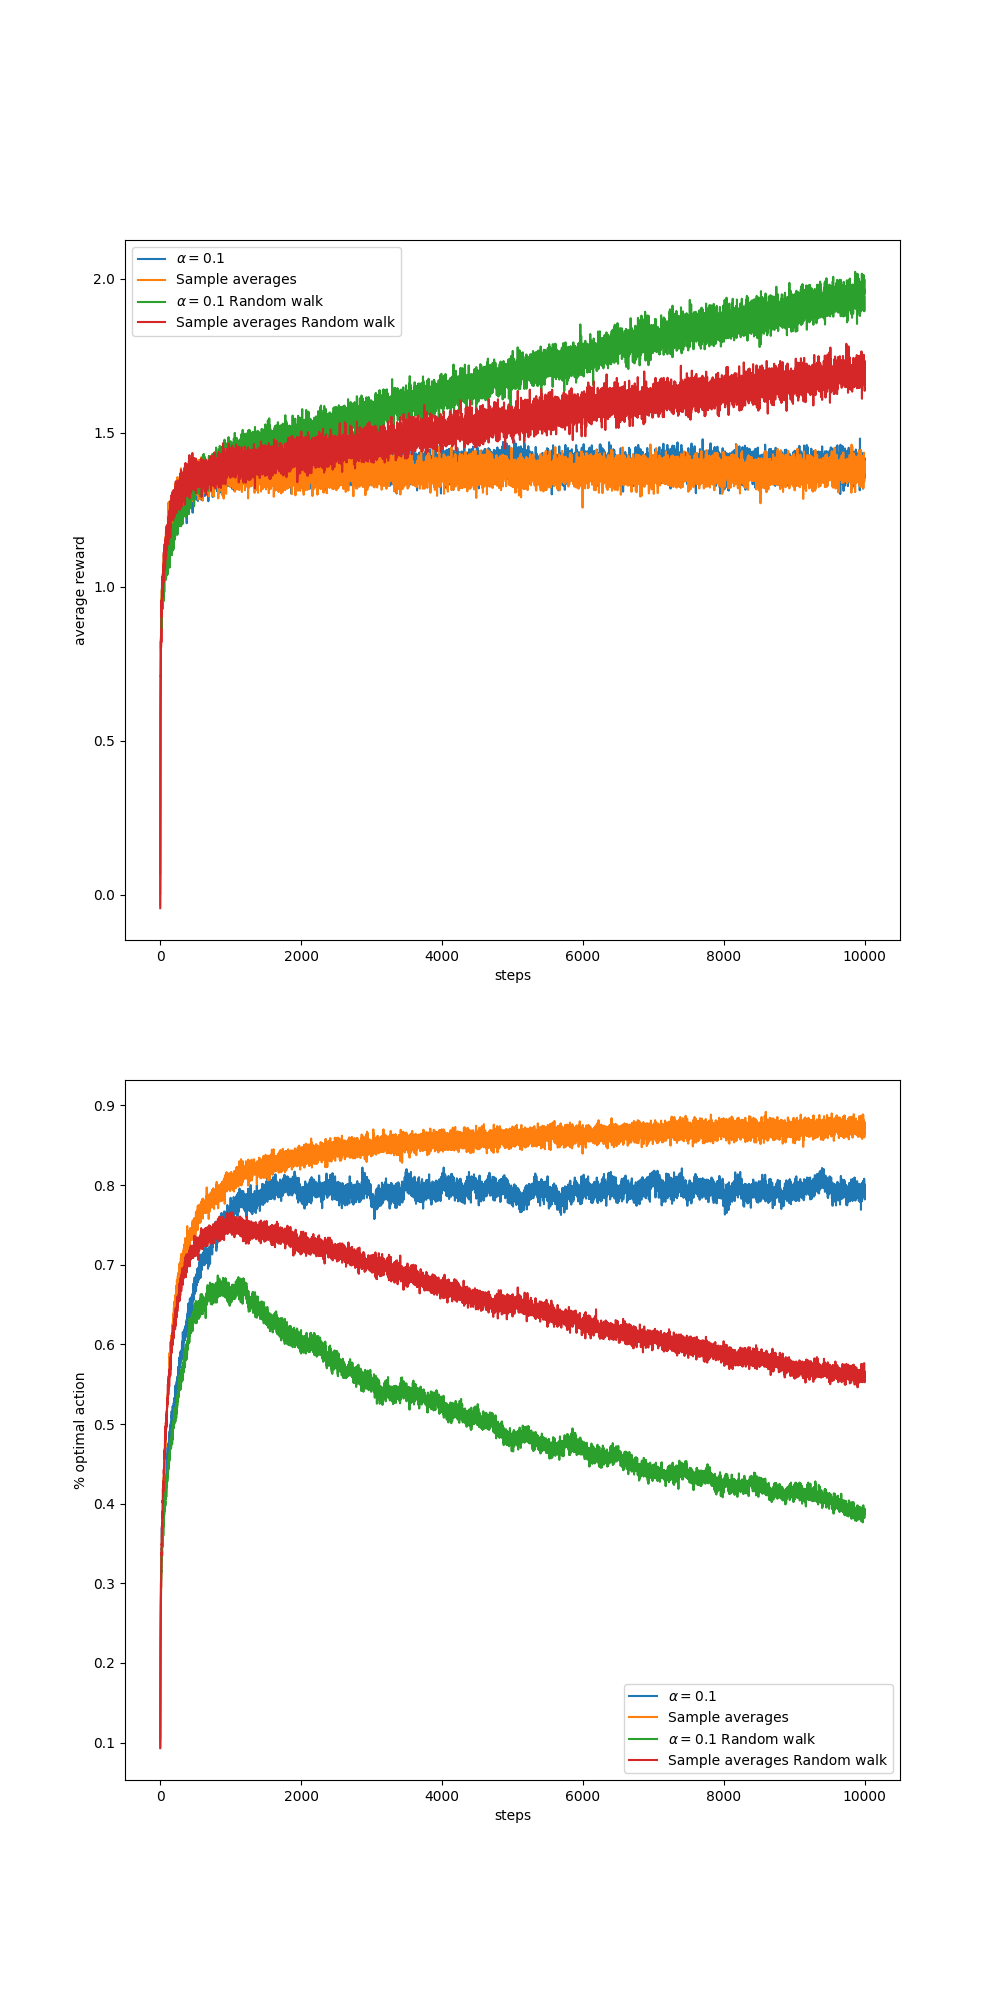
\includegraphics[scale=0.5]{figure_e_2_5}


\end{document}



